\documentclass{article}
\usepackage[utf8]{inputenc}
\setlength{\parskip}{5pt} % esp. entre parrafos
\setlength{\parindent}{0pt} % esp. al inicio de un parrafo
\usepackage{listings} % listings
\usepackage{color} %colores
\usepackage{amsmath} % mates
\usepackage[sort&compress,numbers]{natbib} % referencias
\usepackage{url} % que las URLs se vean lindos
\usepackage[top=15mm,left=20mm,right=20mm,bottom=25mm]{geometry} % margenes
\usepackage{hyperref} % ligas de URLs
\usepackage{graphicx} % poner figuras
\usepackage[spanish,es-tabla]{babel} % nombre tablas


\definecolor{mypink}{rgb}{0.976, 0.462, 0.847}
\definecolor{mygray}{rgb}{0.976, 0.980, 0.980}
\definecolor{myblue}{rgb}{0.258, 0.682, 1}
\definecolor{mypink2}{rgb}{0.525, 0.054, 0.4}
\lstset{ 
  backgroundcolor=\color{mygray},
  commentstyle=\color{myblue},
  keywordstyle=\color{mypink}, 
  numberstyle=\tiny\color{mypink}
  stringstyle=\color{mypink2}, 
  breaklines=true,
}


\title{Tarea 7}
\author{Eduardo Navarro}
\date{Octubre 2021}

\begin{document}

\maketitle

\section{Introducción}

En esta práctica se realizó un estudio sobre el movimiento hacia los máximos dentro de una función dada y acotada.

\section{Desarrollo}

Con las instrucciones de la tarea \cite{busqueda} y lo visto en clase \cite{twitchsimu} se le hicieron modificaciones al código para obtener los máximos \cite{maria} añadiendo información al \texttt{for} que limita la función, a diversos pasos y sus respectivas réplicas con un \texttt{for} para el análisis estadístico de una función dada. Así mismo se creó un gif que muestra el movimiento de los puntos \cite{gif}.

Función \ref{funcion} usada con restricción: $ -1 \leq x, y \leq 6 \ $ 
\begin{equation}
f(x,y) = 10* cos(x^2) - 10 * x + 12 * cos(y^2) -5* y
\label{funcion}
\end{equation}

\begin{lstlisting} [language=R, caption= Código para la obtención de máximos.]
library(lattice)
library(sp)
library(viridisLite)
library(reshape2)

datos<- data.frame()

g <- function(x,y) { # modificamos para que sea interesante
  return((10* cos(x^2) - 10 * x + 12 * cos(y^2) -5* y))
}
x <- seq(-1, 6, 0.4)
y <-  x
z <- outer(x, y, g)

low <- -1
high <- 6
j <- seq(0.25, 4, 0.25)
repe<- (1:30)
replicas <- 50 #puntitos

for (step in j) {
for (rep in repe) {

replica <- function(t) {
  curr <- c(runif(1, low, high), runif(1, low, high))
  best <- curr
  for (tiempo in 1:t) {
    
    delta <- runif(1, 0, step)
    
    left <- curr +c(-delta,0)
    
    right <- curr + c(delta,0)
    
    up <- curr + c(0,-delta)
    
    down <- curr + c(0,delta)
    
    puntos<- c(left,right,up,down)
    
    for(p in 1:8){
      if(puntos[p] < (-1)){
        puntos[p] <- puntos[p]+6 
      }
      if(puntos[p] > 6){
        puntos[p] <- puntos[p]-1
      }
    }
    
    ux<-c()
    uy<-c()
    
    for(q in 1:8){
      if(q %% 2 == 0){
        uy <- c(uy,puntos[q])
      }else{
        ux <- c(ux,puntos[q])
      }
    }
    
    ug<- c()
    
    for(r in 1:4){
      ug <- c(ug, g(ux[r], uy[r]) )
    }
    ppmax <- which.max(ug)
    curr <- c(ux[ppmax], uy[ppmax])
    if(g(curr[1],curr[2]) > g(best[1],best[2])){
    
      best <- curr
    }
  }
  return(best)
}
\end{lstlisting}

\begin{lstlisting}[language=R, caption= Código para la obtención de imágenes.]
for (pot in 1:40) { #numero de imagenes a repeticiones dadas
  tmax <- pot
  resultados <- foreach(i = 1:replicas, .combine=c) %dopar% replica(tmax)

  
ux<- c()
uy<- c()

sal<-(2*replicas)

for(q in 1:sal){
  if(q %% 2 == 0){
    uy <- c(uy,resultados[q])
  }else{
    ux <- c(ux,resultados[q])
  }
}


val <- c()
for(r in 1:replicas){
  val <- c(val, g(ux[r], uy[r]))
}
  
maximo <- which.max(val)
x <- seq(-1, 6, 0.4) 
y <-  x
z <- outer(x, y, g)

dimnames(z) <- list(x, y)
d <- melt(z)
names(d) <- c("x", "y", "z")


png(paste0("t7_", tmax, ".png", sep=""), width=500, height=500)
plot(levelplot(z ~ x * y, data = d))
trellis.focus("panel", 1, 1, highlight=FALSE)
lpoints(ux, uy, pch=1, col="red", cex=2)
trellis.unfocus()
trellis.focus("panel"[1], 1, 1, highlight=FALSE)
lpoints(ux[maximo], uy[maximo], pch=20, col="green",cex=3)
trellis.unfocus()

graphics.off()
}
ultimo<-min(val)
datos<- rbind(datos,c(step,ultimo))
\end{lstlisting}
Se trabajó sobre el gráfico con una proyección 2D del plano sobre el cual observaremos el movimiento gracias a un gif \cite{gif}.


\newpage

\begin{figure} [h!]% figura
\renewcommand{\figurename}{Gráfica}
    \centering
    \caption{ Gráfica 3D de la función.}
    \label{grafica1}
    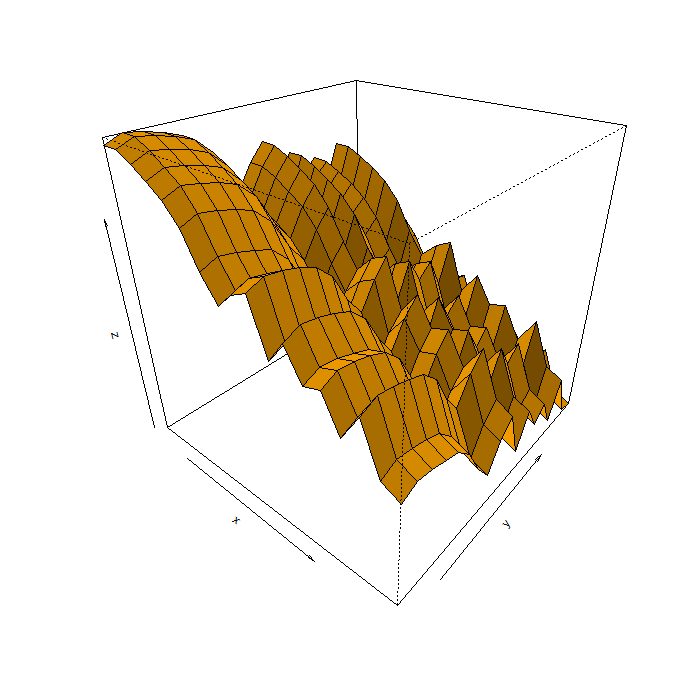
\includegraphics[width=100mm]{grafica1.png} % archivo
\end{figure}


\begin{figure} [h!]% figura
\renewcommand{\figurename}{Gráfica}
    \centering
    \caption{ Gráfica 2D de la función.}
    \label{grafica2}
    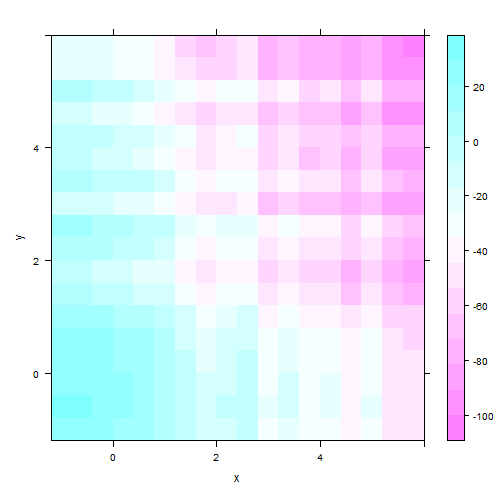
\includegraphics[width=110mm]{grafica2.png} % archivo
\end{figure}

\newpage

Con esto se generaron los datos de la tabla \ref{tabla1} y se le hicieron las correspondientes pruebas estadísticas.

\begin{table}[h!]
\centering
\caption{Ejemplo de datos obtenidos.}
\label{tabla1}
\begin{tabular}{|c|r|}
\hline
Paso & \multicolumn{1}{c|}{Distancia} \\ \hline
0.25 & -56.1624408 \\ \hline
0.25 & -56.2513706 \\ \hline
0.25 & -55.7223354 \\ \hline
0.25 & -62.1704963 \\ \hline
0.25 & -53.4912933 \\ \hline
0.25 & -62.2414052 \\ \hline
0.25 & -56.2131058 \\ \hline
0.25 & -55.7417835 \\ \hline
\end{tabular}
\end{table}

\begin{figure} [h!]% figura
\renewcommand{\figurename}{Gráfica}
    \centering
    \caption{Último Máximo obtenido a partir del tamaño de paso.}
    \label{grafica3}
    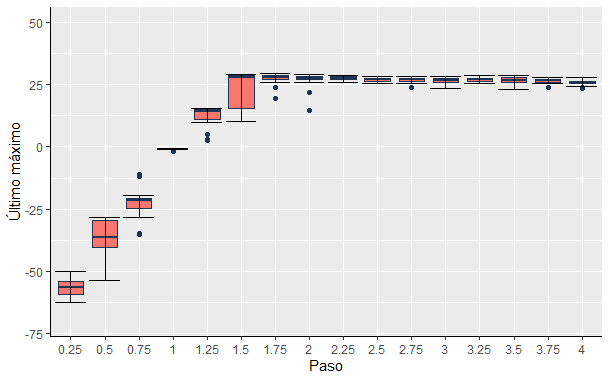
\includegraphics[width=100mm]{grafica3.png} % archivo
\end{figure}

\begin{lstlisting} [language=R, caption= Código para la obtención de la gráfica y pruebas estadísticas.]
library(ggplot2)
library(tidyverse)

names(datos)<-c("paso", "distancia")
datos$paso = as.factor(datos$paso)

ggplot(datos, aes(x=paso , y= distancia , fill= rep)) + # fill=name allow to automatically dedicate a color for each group
  geom_boxplot(fill = "#F8766D", colour = "#1F3552")+
  stat_boxplot(geom = "errorbar", width = 0.9)+
  theme(axis.line = element_line(colour = "black", size = 0.25))+
  coord_cartesian(ylim = c(-70, 50))+
  labs(x="Paso", y= "Ultimo maximo")

datos%>%
  group_by(paso) %>%
  summarise(
    
    promedio = mean(distancia, na.rm = TRUE),
    desviacion_std = sd(distancia, na.rm = TRUE),
    varianza = sd(distancia, na.rm = TRUE)^2,
    mediana = median(distancia, na.rm = TRUE),
    rango_intercuartil = IQR(distancia, na.rm = TRUE)
  )

tapply(datos$distancia, datos$paso, shapiro.test)

kruskal.test(distancia~paso, data=datos)

pairwise.wilcox.test(datos$distancia, datos$paso)
\end{lstlisting}

De la gráfica \ref{grafica3} podemos observar un máximo efectivo en cuanto al paso del cual después no hay una diferencia notable. Esto se comprueba con las pruebas estadísticas de Shapiro  Wilk \cite{shapiro} y Kruskal Wallis \cite{Kruskall} además de que con la prueba Wilcox \cite{pruebass} se pueden apreciar las diferencias entre grupos.


\begin{table}[h!]
\centering
\caption{Estadísticas obtenidas de la tabla \ref{tabla1}.}
\label{tabla2}
\begin{tabular}{|c|r|r|r|r|r|}
\hline
Paso & \multicolumn{1}{c|}{Promedio} & \multicolumn{1}{c|}{Desviación std} & \multicolumn{1}{c|}{Varianza} & \multicolumn{1}{c|}{Mediana} & \multicolumn{1}{c|}{Rango intercuartil} \\ \hline
0.25 & -56.8 & 3.5 & 12.2 & -56.2 & 5.11 \\ \hline
0.5 & -36.3 & 6.43 & 41.3 & -36.3 & 10.8 \\ \hline
0.75 & -21.2 & 6.21 & 38.6 & -21.5 & 3.9 \\ \hline
1 & -0.966 & 0.281 & 0.0792 & -0.899 & 0.221 \\ \hline
1.25 & 12.6 & 3.6 & 12.9 & 14.4 & 3.95 \\ \hline
1.5 & 23.1 & 6.96 & 48.4 & 27.9 & 13.2 \\ \hline
1.75 & 27.5 & 1.89 & 3.57 & 28 & 1.44 \\ \hline
2 & 27 & 2.7 & 7.3 & 27.6 & 1.54 \\ \hline
2.25 & 27.6 & 0.659 & 0.434 & 27.6 & 0.992 \\ \hline
2.5 & 26.9 & 0.793 & 0.629 & 27 & 1.21 \\ \hline
2.75 & 26.7 & 0.913 & 0.834 & 26.8 & 1.14 \\ \hline
3 & 26.6 & 1.25 & 1.56 & 26.8 & 1.68 \\ \hline
3.25 & 26.9 & 0.777 & 0.604 & 27 & 1.31 \\ \hline
3.5 & 26.6 & 1.41 & 1.99 & 26.8 & 1.86 \\ \hline
3.75 & 26.5 & 0.875 & 0.766 & 26.6 & 1.06 \\ \hline
4 & 25.9 & 0.986 & 0.973 & 26 & 0.977 \\ \hline
\end{tabular}
\end{table}

\begin{table}[h!]
\centering
\caption{Resultados de la prueba Shapiro–Wilk para la tabla \ref{tabla1}.}
\label{tabla3}
\begin{tabular}{|c|r|r|}
\hline
Paso & \multicolumn{1}{c|}{W} & \multicolumn{1}{c|}{P} \\ \hline
0.25 & 0.91671 & 0.02206 \\ \hline
0.5 & 0.92926 & 0.04694 \\ \hline
0.75 & 0.88267 & 0.003249 \\ \hline
1 & 0.73805 & $5.87\times 10^{-6}$ \\ \hline
1.25 & 0.73931 & $6.15\times 10^{-6}$ \\ \hline
1.5 & 0.74202 & $6.78\times 10^{-6}$ \\ \hline
1.75 & 0.70755 & $2.01\times 10^{-6}$ \\ \hline
2 & 0.54997 & $1.89\times 10^{-8}$ \\ \hline
2.25 & 0.94227 & 0.1047 \\ \hline
2.5 & 0.96461 & 0.404 \\ \hline
2.75 & 0.94005 & 0.09125 \\ \hline
3 & 0.9346 & 0.06513 \\ \hline
3.25 & 0.95696 & 0.2586 \\ \hline
3.5 & 0.92479 & 0.03577 \\ \hline
3.75 & 0.95538 & 0.2351 \\ \hline
4 & 0.95128 & 0.183 \\ \hline
\end{tabular}
\end{table}

\newpage

\begin{table}[h!]
\centering
\caption{Resultados de la prueba Kruskal-Wallis para la tabla \ref{tabla1}.}
\label{tabla4}
 \begin{tabular}{|c|c|c|}
    \hline
   H(15) & p-value \\
    \hline
    349.49 & $2.2\times 10^{-16}$ \\
    \hline
\end{tabular}
\end{table}

\begin{table}[h!]
\centering
\caption{Resultados de la prueba por parejas de Wilcox para la tabla \ref{tabla1}.}
\label{tabla5}
\begin{tabular}{|c|r|r|r|r|r|r|r|c|}
\hline
 & \multicolumn{1}{c|}{0.25} & \multicolumn{1}{c|}{0.5} & \multicolumn{1}{c|}{0.75} & \multicolumn{1}{c|}{1} & \multicolumn{1}{c|}{1.25} & \multicolumn{1}{c|}{1.5} & \multicolumn{1}{c|}{1.75} & 2 \\ \hline
0.5 & $6.7\times 10^{-14}$ & \multicolumn{1}{c|}{-} & \multicolumn{1}{c|}{-} & \multicolumn{1}{c|}{-} & \multicolumn{1}{c|}{-} & \multicolumn{1}{c|}{-} & \multicolumn{1}{c|}{-} & - \\ \hline
0.75 & $2\times 10^{-15}$ & $5.6\times 10^{-12}$ & \multicolumn{1}{c|}{-} & \multicolumn{1}{c|}{-} & \multicolumn{1}{c|}{-} & \multicolumn{1}{c|}{-} & \multicolumn{1}{c|}{-} & - \\ \hline
1 & $2\times 10^{-15}$ & $2\times 10^{-15}$ & $2\times 10^{-15}$ & \multicolumn{1}{c|}{-} & \multicolumn{1}{c|}{-} & \multicolumn{1}{c|}{-} & \multicolumn{1}{c|}{-} & - \\ \hline
1.25 & $2\times 10^{-15}$ & $2\times 10^{-15}$ & $2\times 10^{-15}$ & $2\times 10^{-15}$ & \multicolumn{1}{c|}{-} & \multicolumn{1}{c|}{-} & \multicolumn{1}{c|}{-} & - \\ \hline
1.5 & $2\times 10^{-15}$ & $2\times 10^{-15}$ & $2\times 10^{-15}$ & $2\times 10^{-15}$ & $3.2\times 10^{-7}$ & \multicolumn{1}{c|}{-} & \multicolumn{1}{c|}{-} & - \\ \hline
1.75 & $2\times 10^{-15}$ & $2\times 10^{-15}$ & $2\times 10^{-15}$ & $2\times 10^{-15}$ & $2\times 10^{-15}$ & 1 & \multicolumn{1}{c|}{-} & - \\ \hline
2 & $2\times 10^{-15}$ & $2\times 10^{-15}$ & $2\times 10^{-15}$ & $2\times 10^{-15}$ & $1.9\times 10^{-13}$ & 1 & 1 & - \\ \hline
2.25 & $2\times 10^{-15}$ & $2\times 10^{-15}$ & $2\times 10^{-15}$ & $2\times 10^{-15}$ & $2\times 10^{-15}$ & 1 & 1 & \multicolumn{1}{r|}{1} \\ \hline
2.5 & $2\times 10^{-15}$ & $2\times 10^{-15}$ & $2\times 10^{-15}$ & $2\times 10^{-15}$ & $2\times 10^{-15}$ & 1 & 0.0533 & \multicolumn{1}{r|}{0.3255} \\ \hline
2.75 & $2\times 10^{-15}$ & $2\times 10^{-15}$ & $2\times 10^{-15}$ & $2\times 10^{-15}$ & $2\times 10^{-15}$ & 1 & 0.0221 & \multicolumn{1}{r|}{0.0759} \\ \hline
3 & $2\times 10^{-15}$ & $2\times 10^{-15}$ & $2\times 10^{-15}$ & $2\times 10^{-15}$ & $2\times 10^{-15}$ & 1 & 0.0259 & \multicolumn{1}{r|}{0.2118} \\ \hline
3.25 & $2\times 10^{-15}$ & $2\times 10^{-15}$ & $2\times 10^{-15}$ & $2\times 10^{-15}$ & $2\times 10^{-15}$ & 1 & 0.0501 & \multicolumn{1}{r|}{0.2643} \\ \hline
3.5 & $2\times 10^{-15}$ & $2\times 10^{-15}$ & $2\times 10^{-15}$ & $2\times 10^{-15}$ & $2\times 10^{-15}$ & 1 & 0.0579 & \multicolumn{1}{r|}{0.2808} \\ \hline
3.75 & $2\times 10^{-15}$ & $2\times 10^{-15}$ & $2\times 10^{-15}$ & $2\times 10^{-15}$ & $2\times 10^{-15}$ & 1 & 0.0021 & \multicolumn{1}{r|}{0.0077} \\ \hline
4 & $2\times 10^{-15}$ & $2\times 10^{-15}$ & $2\times 10^{-15}$ & $2\times 10^{-15}$ & $2\times 10^{-15}$ & 1 & $1.1\times 10^{-5}$ & \multicolumn{1}{r|}{$4.3\times 10^{-5}$} \\ \hline
\end{tabular}
\end{table}

\begin{table}[h!]
\centering
\caption{Resultados de la prueba por parejas de Wilcox para la tabla \ref{tabla1} continuación.}
\label{tabla6}
\begin{tabular}{|c|c|c|c|c|c|c|c|}
\hline
\multicolumn{1}{|l|}{} & 2.25 & 2.5 & 2.75 & 3 & 3.25 & 3.5 & 3.75 \\ \hline
0.5 & - & - & - & - & - & - & - \\ \hline
0.75 & - & - & - & - & - & - & - \\ \hline
1 & - & - & - & - & - & - & - \\ \hline
1.25 & - & - & - & - & - & - & - \\ \hline
1.5 & - & - & - & - & - & - & - \\ \hline
1.75 & - & - & - & - & - & - & - \\ \hline
2 & - & - & - & - & - & - & - \\ \hline
2.25 & - & - & - & - & - & - & - \\ \hline
2.5 & \multicolumn{1}{r|}{0.0517} & - & - & - & - & - & - \\ \hline
2.75 & \multicolumn{1}{r|}{0.0031} & \multicolumn{1}{r|}{1} & - & - & - & - & - \\ \hline
3 & \multicolumn{1}{r|}{0.0269} & \multicolumn{1}{r|}{1} & \multicolumn{1}{r|}{1} & - & - & - & - \\ \hline
3.25 & \multicolumn{1}{r|}{0.0409} & \multicolumn{1}{r|}{1} & \multicolumn{1}{r|}{1} & \multicolumn{1}{r|}{1} & - & - & - \\ \hline
3.5 & \multicolumn{1}{r|}{0.0629} & \multicolumn{1}{r|}{1} & \multicolumn{1}{r|}{1} & \multicolumn{1}{r|}{1} & \multicolumn{1}{r|}{1} & - & - \\ \hline
3.75 & \multicolumn{1}{r|}{$2.7\times 10^{-5}$} & \multicolumn{1}{r|}{1} & \multicolumn{1}{r|}{1} & \multicolumn{1}{r|}{1} & \multicolumn{1}{r|}{1} & \multicolumn{1}{r|}{1} & - \\ \hline
4 & \multicolumn{1}{r|}{$2.7\times 10^{-8}$} & \multicolumn{1}{r|}{0.0033} & \multicolumn{1}{r|}{0.0333} & \multicolumn{1}{r|}{0.2369} & \multicolumn{1}{r|}{0.0043} & \multicolumn{1}{r|}{0.3958} & \multicolumn{1}{l|}{0.3922} \\ \hline
\end{tabular}
\end{table}

\section{Conclusiones}
Con los resultados obtenidos podemos concluir que el paso influye en el máximo a obtener debido a que a mayor paso más distancia se recorre y esto le permite alcanzar sin tanta dificultad el punto mas alto. Con el gif se pudo observar el movimiento de los puntos alrededor de la superficie de la gráfica. En base a las pruebas estadísticas podemos concluir que a partir del paso 1.75 se obtiene la mejor velocidad para alcanzar el máximo ya que no hubo mejoras notables después de este paso. 

\bibliography{referencias}
\bibliographystyle{plainnat}
\end{document}

